% =============================================================================
%  Diplomado en Data Science Aplicada con Python para la Toma de Decisiones
%  Clase 32: Series Temporales II - De la Estacionariedad a la Decision
%  Arca Continental Ecuador | UDLA
% =============================================================================
\documentclass[aspectratio=169, 11pt]{beamer}

\usepackage[T1]{fontenc}
\usepackage[utf8]{inputenc}
\usepackage[spanish,es-noshorthands]{babel}
\usepackage{FiraSans}
\usepackage{FiraMono}
\renewcommand{\familydefault}{\sfdefault}
\usepackage{graphicx}
\usepackage{tikz}
\usetikzlibrary{arrows.meta, positioning, shapes.geometric, shapes.misc,
  calc, fit, decorations.pathreplacing, backgrounds}
\usepackage{fontawesome5}
\usepackage{minted}
\usepackage{tcolorbox}
\tcbuselibrary{minted, skins, breakable}
\usepackage{booktabs}
\usepackage{colortbl}
\usepackage{multicol}
\usepackage{hyperref}
\usepackage{calc}
\usepackage{amsmath}

\definecolor{arcaRed}{HTML}{C82B40}
\definecolor{arcaDark}{HTML}{6B1525}
\definecolor{udlaCrimson}{HTML}{A31545}
\definecolor{arcaGray}{HTML}{F5F5F5}
\definecolor{arcaLightGray}{HTML}{EBEBEB}
\definecolor{textDark}{HTML}{2D2D2D}
\definecolor{textMuted}{HTML}{6B7280}
\definecolor{codeGreen}{HTML}{16A34A}
\definecolor{codeBlue}{HTML}{2563EB}
\definecolor{codeOrange}{HTML}{EA580C}
\definecolor{codePurple}{HTML}{7C3AED}

\usetheme{default}
\usecolortheme{default}
\setbeamertemplate{navigation symbols}{}
\setbeamertemplate{footline}{}
\setbeamertemplate{headline}{}
\setbeamercolor{normal text}{fg=textDark}
\setbeamercolor{frametitle}{fg=arcaRed, bg=white}
\setbeamercolor{title}{fg=white}
\setbeamercolor{subtitle}{fg=white!85}
\setbeamercolor{author}{fg=white!80}
\setbeamercolor{date}{fg=white!70}
\setbeamercolor{item}{fg=arcaRed}
\setbeamercolor{subitem}{fg=arcaDark}
\setbeamercolor{block title}{fg=white, bg=arcaRed}
\setbeamercolor{block body}{fg=textDark, bg=arcaGray}
\setbeamercolor{section in toc}{fg=arcaDark}
\setbeamerfont{frametitle}{size=\Large, series=\bfseries}
\setbeamerfont{title}{size=\huge, series=\bfseries}
\setbeamerfont{subtitle}{size=\large}
\setbeamerfont{author}{size=\normalsize}
\setbeamerfont{date}{size=\small}
\setbeamerfont{block title}{size=\normalsize, series=\bfseries}
\setbeamerfont{footnote}{size=\tiny}
\setbeamertemplate{itemize item}{\scriptsize\raise1.5pt\hbox{\color{arcaRed}$\blacktriangleright$}}
\setbeamertemplate{itemize subitem}{\scriptsize\raise1pt\hbox{\color{arcaDark}$\bullet$}}
\setbeamertemplate{enumerate items}[default]
\setbeamercolor{enumerate item}{fg=arcaRed}

\setbeamertemplate{headline}{%
  \begin{tikzpicture}[remember picture, overlay]
    \fill[arcaDark] (current page.north west) rectangle
      ([yshift=-0.7cm]current page.north east);
    \node[anchor=west, inner sep=0pt] at
      ([xshift=0.6cm, yshift=-0.35cm]current page.north west)
      {
\includegraphics[height=0.45cm]{../logo_udla_white.png}};
    \node[anchor=east, inner sep=0pt] at
      ([xshift=-0.6cm, yshift=-0.35cm]current page.north east)
      {
\includegraphics[height=0.45cm]{../ArcaContinental_white.png}};
  \end{tikzpicture}%
  \vspace{0.7cm}%
}

\setbeamertemplate{footline}{%
  \begin{tikzpicture}[remember picture, overlay]
    \node[anchor=south east, font=\scriptsize\bfseries\color{arcaRed}] at
      ([xshift=-0.5cm, yshift=0.15cm]current page.south east)
      {\insertframenumber};
  \end{tikzpicture}%
  \vspace{0.3cm}%
}

\setbeamertemplate{frametitle}{%
  \vspace{0.25cm}%
  \usebeamerfont{frametitle}\usebeamercolor[fg]{frametitle}\insertframetitle%
  \par\vspace{2pt}%
  \begin{tikzpicture}
    \fill[arcaRed] (0,0) rectangle (3cm, 1.5pt);
    \fill[arcaLightGray] (3cm,0) rectangle (\textwidth, 0.5pt);
  \end{tikzpicture}%
  \vspace{0.1cm}%
}

\newtcblisting{pyblock}[1][]{%
  listing engine=minted, minted language=python, minted style=friendly,
  minted options={fontsize=\small, linenos=false, breaklines=true, python3=true},
  colback=arcaGray, colframe=arcaRed, left=4pt, right=4pt, top=4pt, bottom=4pt,
  boxrule=0pt, leftrule=3pt, arc=2pt, listing only, #1}

\newcommand{\sectionframe}[2]{%
  \begingroup
  \setbeamertemplate{headline}{}%
  \setbeamertemplate{footline}{}%
  \begin{frame}[plain, noframenumbering]
    \begin{tikzpicture}[remember picture, overlay]
      \fill[arcaRed] (current page.south west) rectangle (current page.north east);
      \node[anchor=center, text=white, font=\Huge\bfseries, text width=12cm,
            align=center] at ([yshift=0.5cm]current page.center) {#1};
      \node[anchor=center, text=white!80, font=\large, text width=10cm,
            align=center] at ([yshift=-0.8cm]current page.center) {#2};
    \end{tikzpicture}
  \end{frame}
  \endgroup
}

\title{Diplomado en Data Science Aplicada\\con Python para la Toma de Decisiones}
\subtitle{Clase 32: Series Temporales II --- de la Estacionariedad a la Decision}
\author{Carlos Enrique Mosquera Trujillo}
\date{26 de Mayo, 2026}

\begin{document}

% =============================================================================
%  PORTADA
% =============================================================================
{
\setbeamertemplate{headline}{}
\setbeamertemplate{footline}{}
\begin{frame}[plain, noframenumbering]
  \begin{tikzpicture}[remember picture, overlay]
    \fill[arcaDark] (current page.south west) rectangle (current page.north east);
    \fill[arcaRed] ([yshift=-3.5cm]current page.north west) rectangle
      ([yshift=-4.2cm]current page.north east);
    \node[anchor=west, inner sep=0pt] at
      ([xshift=1cm, yshift=-1.5cm]current page.north west)
      {
\includegraphics[height=1cm]{../logo_udla_white.png}};
    \node[anchor=east, inner sep=0pt] at
      ([xshift=-1cm, yshift=-1.5cm]current page.north east)
      {
\includegraphics[height=1cm]{../ArcaContinental_white.png}};
  \end{tikzpicture}
  \vspace{2.5cm}
  \begin{center}
    {\usebeamerfont{title}\usebeamercolor[fg]{title}\inserttitle\par}
    \vspace{0.4cm}
    {\usebeamerfont{subtitle}\usebeamercolor[fg]{subtitle}\insertsubtitle\par}
    \vspace{0.6cm}
    {\usebeamerfont{author}\usebeamercolor[fg]{author}\insertauthor\par}
    \vspace{0.15cm}
    {\usebeamerfont{date}\usebeamercolor[fg]{date}\insertdate\par}
  \end{center}
\end{frame}
}

% =============================================================================
%  BLOQUE 0 - El problema general de la planeacion
% =============================================================================
\sectionframe{Bloque 0}{El problema universal\\de toda planeacion de demanda}

\begin{frame}[shrink]{Donde quedamos en clase 31}
  \vspace{6pt}
  {\footnotesize\color{arcaDark}Los ladrillos que ya tenemos:\par}
  \vspace{6pt}
  \begin{itemize}\setlength{\itemsep}{4pt}
    \footnotesize
    \item Serie temporal = secuencia de observaciones indexadas por tiempo.
    \item \textbf{Naive} y \textbf{media movil}: dos modelos cero que sirven como baseline.
    \item \textbf{Descomposicion}: tendencia + estacionalidad + residuo.
    \item \textbf{Estacionariedad}: pregunta que dejamos abierta.
    \item \textbf{Diferenciacion}: la introdujimos pero no la motivamos bien.
    \item \textbf{ADF}: una herramienta de diagnostico que vimos rapido.
  \end{itemize}
  \vspace{8pt}
  \begin{tcolorbox}[colback=arcaRed!8, colframe=arcaRed, leftrule=3pt,
    boxrule=0pt, sharp corners, left=8pt, right=8pt, top=4pt, bottom=4pt]
    {\small\color{arcaDark}\bfseries
    Hoy retomamos estacionariedad y diferenciacion con verdadera motivacion,
    aprendemos Prophet en accion, y cerramos aplicandolo a un caso real.}
  \end{tcolorbox}
\end{frame}

\begin{frame}[shrink]{El problema universal de la planeacion de demanda}
  \begin{center}
    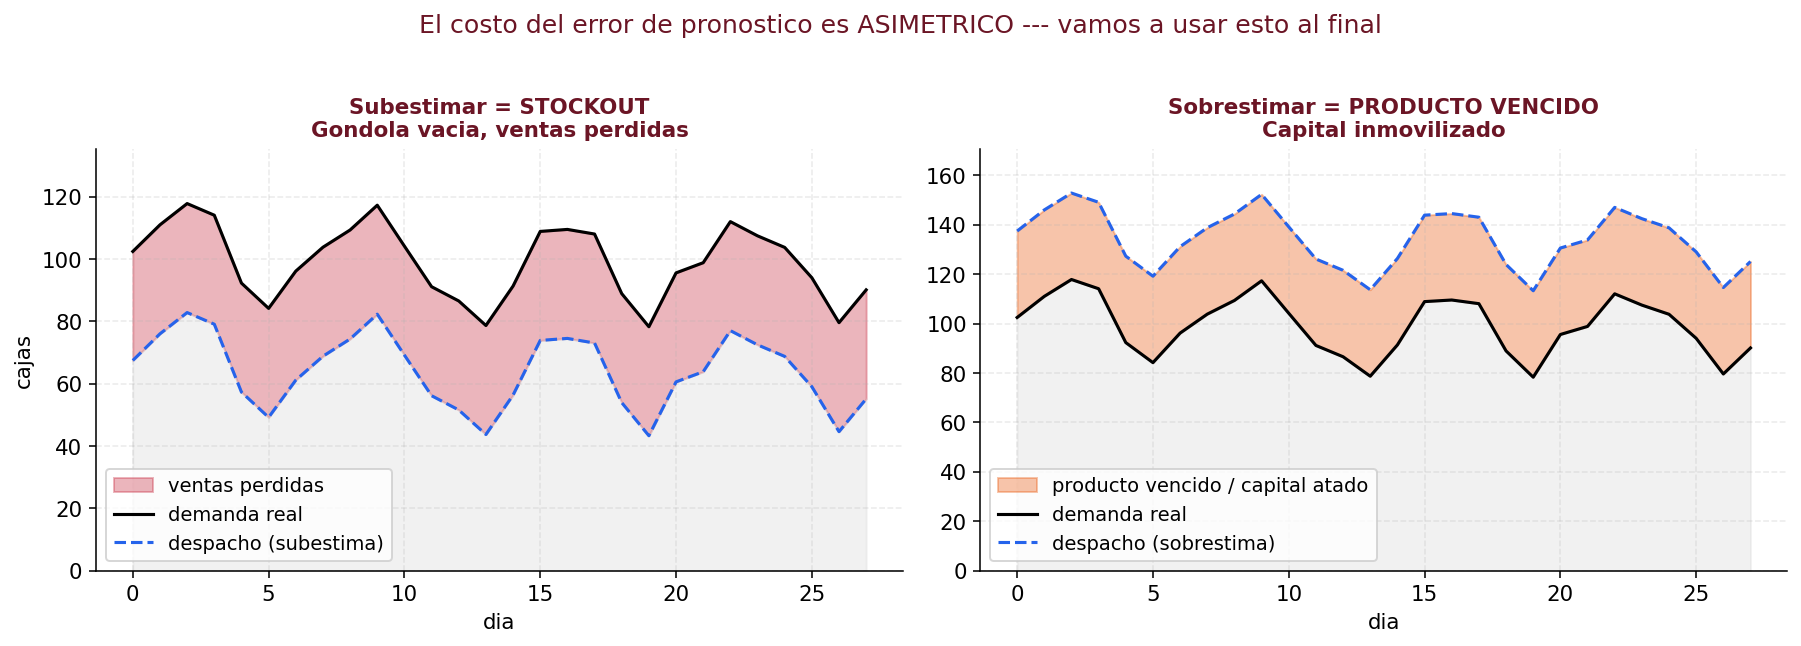
\includegraphics[width=0.97\textwidth]{fig_problema_planeacion.png}
  \end{center}
  \vspace{2pt}
  \begin{tcolorbox}[colback=arcaGray, colframe=arcaRed, leftrule=3pt,
    boxrule=0pt, sharp corners, left=8pt, right=8pt, top=4pt, bottom=4pt]
    {\footnotesize\color{arcaDark}
    Cualquier persona que planea inventario, capacidad, personal o presupuesto
    enfrenta este dilema. El costo del error NO es simetrico. Recuerda este
    concepto: al final de la clase vamos a usarlo para convertir una prediccion
    en una DECISION.}
  \end{tcolorbox}
\end{frame}

\begin{frame}[shrink]{Plan de la clase de hoy}
  \begin{enumerate}\setlength{\itemsep}{4pt}
    \footnotesize
    \item[\textbf{1.}] \textbf{Por que estacionariedad} --- experimento de descubrimiento.
    \item[\textbf{2.}] \textbf{Diferenciacion} --- la cirugia que vuelve estacionaria una serie.
    \item[\textbf{3.}] \textbf{Prophet en accion} --- sobre AirPassengers, dataset clasico.
    \item[\textbf{4.}] \textbf{Metricas honestas} --- MAE, RMSE, MAPE, WAPE y walk-forward CV.
    \item[\textbf{5.}] \textbf{Inferencia} --- de prediccion a decision via costo asimetrico.
    \item[\textbf{6.}] \textbf{Caso aplicado} --- Favorita Quito Q44, forecast de 6 meses.
    \item[\textbf{7.}] \textbf{Cierre} --- decision tree y que viene en clase 33 (redes).
  \end{enumerate}
  \vspace{6pt}
  {\footnotesize\color{arcaDark}\bfseries
  Trabajamos primero sobre series simples y conocidas. Solo cuando dominamos la herramienta
  la aplicamos al caso real.}
\end{frame}

% =============================================================================
%  BLOQUE 1 - POR QUE ESTACIONARIEDAD
% =============================================================================
\sectionframe{Bloque 1}{Por que un modelo necesita\\que la serie sea estacionaria}

\begin{frame}[shrink]{Mira ambas series y piensa en voz alta}
  \begin{center}
    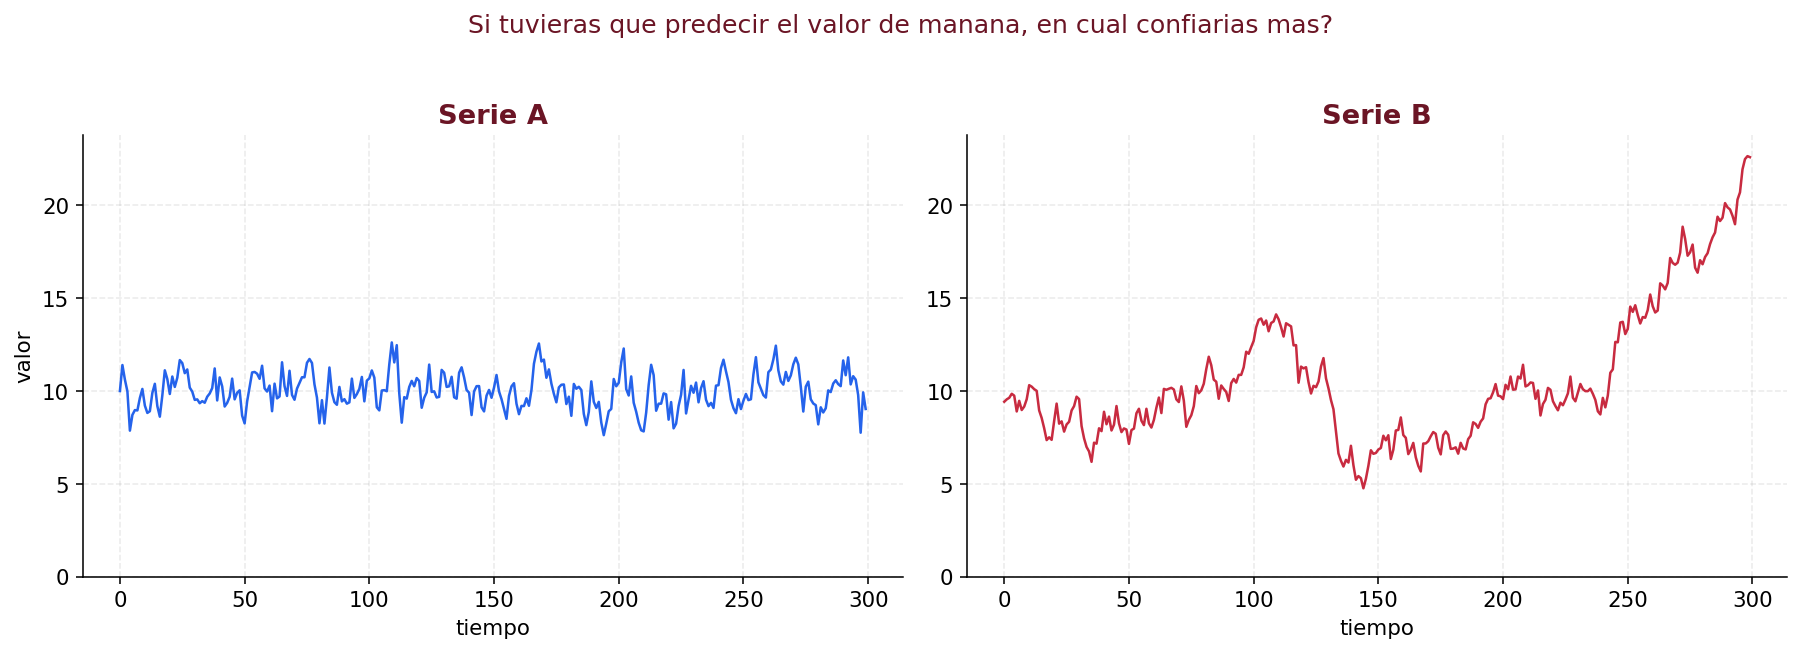
\includegraphics[width=0.95\textwidth]{fig_dos_series_descubrimiento.png}
  \end{center}
  \vspace{4pt}
  \begin{tcolorbox}[colback=arcaGray, colframe=arcaRed, leftrule=3pt,
    boxrule=0pt, sharp corners, left=8pt, right=8pt, top=4pt, bottom=4pt]
    {\footnotesize\color{arcaDark}
    \textbf{Pregunta para el aula:} si tuvieras que predecir el valor de manana,
    en cual de las dos series confiarias mas? Por que?}
  \end{tcolorbox}
\end{frame}

\begin{frame}[shrink]{La respuesta --- la distribucion estable es predecible}
  \begin{center}
    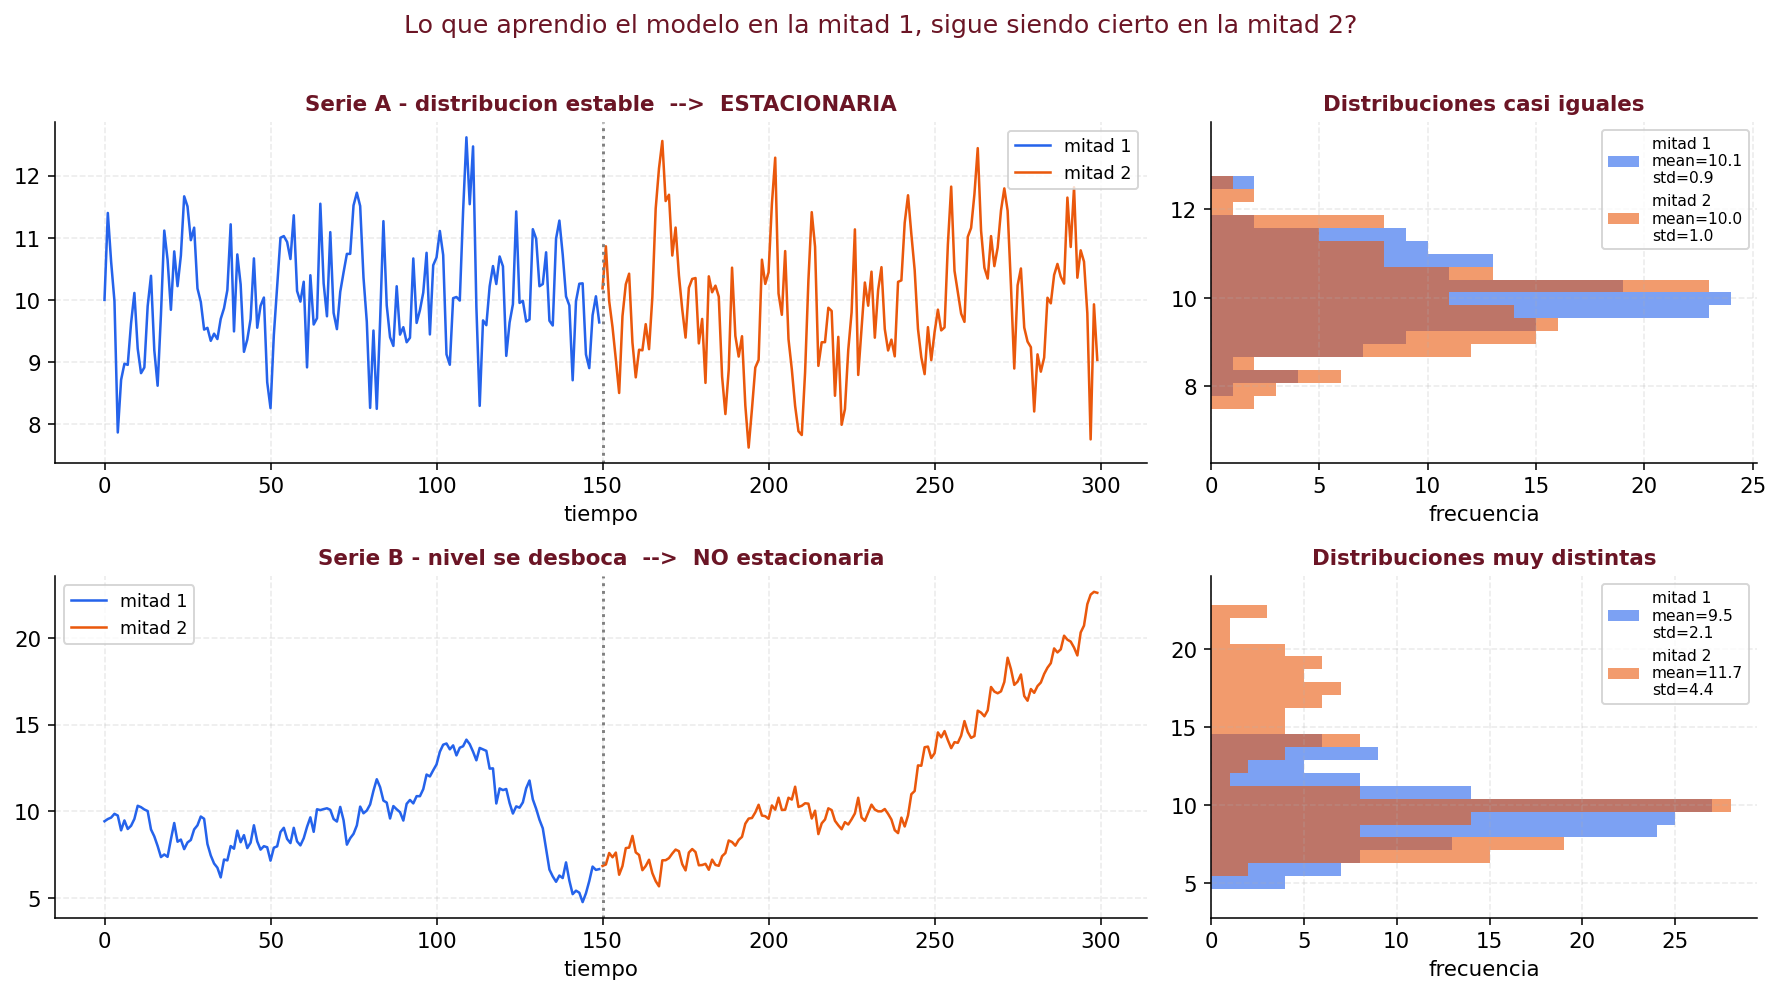
\includegraphics[width=0.97\textwidth]{fig_dos_series_respuesta.png}
  \end{center}
  \vspace{2pt}
  {\footnotesize\color{arcaDark}
  \textbf{Estacionaria} = la distribucion estadistica (media, varianza, autocorrelacion)
  NO cambia con el tiempo. Lo que aprendimos en la mitad 1, sigue siendo cierto en la mitad 2.}
\end{frame}

\begin{frame}[shrink]{Por que importa --- el modelo aprende patrones del pasado}
  \begin{center}
    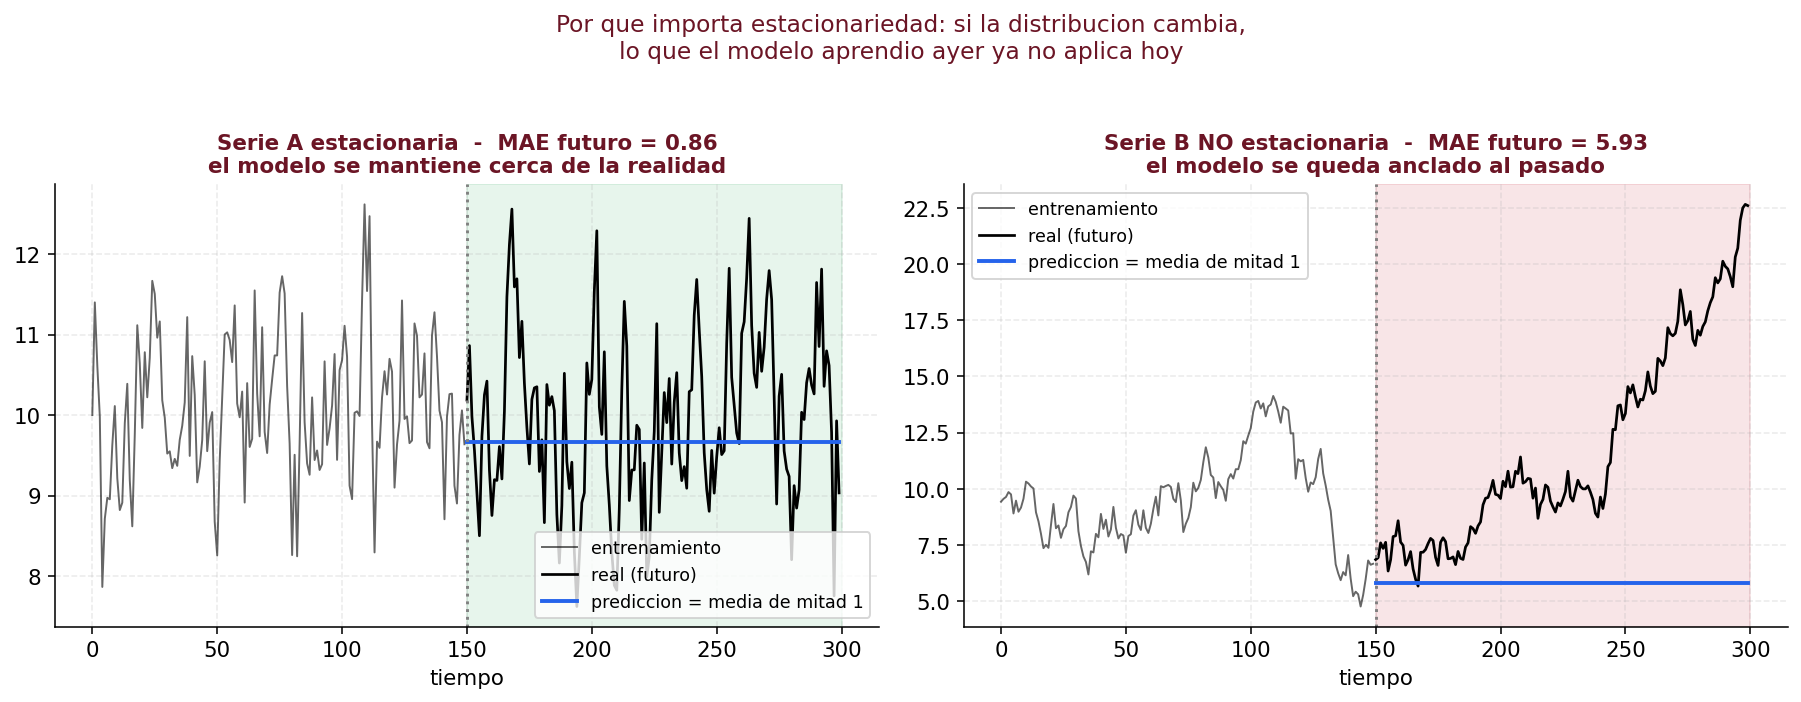
\includegraphics[width=0.95\textwidth]{fig_modelo_falla.png}
  \end{center}
  \vspace{2pt}
  \begin{tcolorbox}[colback=arcaRed!8, colframe=arcaRed, leftrule=3pt,
    boxrule=0pt, sharp corners, left=8pt, right=8pt, top=4pt, bottom=4pt]
    {\footnotesize\color{arcaDark}\bfseries
    Si la distribucion cambia, lo que el modelo aprendio AYER ya no aplica HOY.
    Esa es la razon de fondo por la que pedimos estacionariedad.}
  \end{tcolorbox}
\end{frame}

\begin{frame}[shrink]{Definicion practica}
  \begin{tcolorbox}[colback=arcaGray, colframe=arcaRed, leftrule=3pt,
    boxrule=0pt, sharp corners, left=8pt, right=8pt, top=6pt, bottom=6pt]
    {\small\color{arcaDark}
    Una serie es \textbf{estacionaria} si cumple las tres condiciones:\par}
    \begin{enumerate}\setlength{\itemsep}{4pt}
      \small
      \item \textbf{Media constante} en el tiempo (no hay tendencia).
      \item \textbf{Varianza constante} en el tiempo (no se ``ensancha'' ni se ``angosta'').
      \item \textbf{Autocorrelacion constante}: la relacion entre $y_t$ y $y_{t-k}$
      depende solo de $k$, no del momento en que estemos.
    \end{enumerate}
  \end{tcolorbox}
  \vspace{6pt}
  {\footnotesize\color{arcaDark}
  Casi ninguna serie del mundo real es estacionaria de regalo. Pero hay
  diagnostico (\textbf{ADF}) y una transformacion (\textbf{diferenciar}) para conseguirla.}
\end{frame}

\begin{frame}[fragile, shrink]{ADF --- la prueba estadistica que da una respuesta clara}
  \begin{tcolorbox}[colback=arcaGray, colframe=arcaRed, leftrule=3pt,
    boxrule=0pt, sharp corners, left=8pt, right=8pt, top=4pt, bottom=4pt]
    {\footnotesize\color{arcaDark}
    \textbf{Augmented Dickey-Fuller (ADF):}\par
    \vspace{2pt}
    Hipotesis nula $H_0$: la serie NO es estacionaria.\par
    Si $p < 0.05$: rechazamos $H_0$ $\Rightarrow$ la serie ES estacionaria.\par
    Si $p \geq 0.05$: no rechazamos $\Rightarrow$ tratamos como NO estacionaria.}
  \end{tcolorbox}
  \vspace{6pt}
  \begin{pyblock}
from statsmodels.tsa.stattools import adfuller
stat, p_value, *_ = adfuller(serie.dropna())
print(f"ADF p = {p_value:.3f}")
  \end{pyblock}
  \vspace{4pt}
  {\footnotesize\color{arcaDark}
  ADF no es magia: solo testea cierto tipo de no-estacionariedad (unit root).
  Pero como diagnostico inicial es el estandar de la industria.}
\end{frame}

% =============================================================================
%  BLOQUE 2 - DIFERENCIACION
% =============================================================================
\sectionframe{Bloque 2}{Diferenciacion --- la cirugia\\que vuelve estacionaria una serie}

\begin{frame}[shrink]{La idea central --- modela el CAMBIO, no el VALOR}
  \begin{center}
    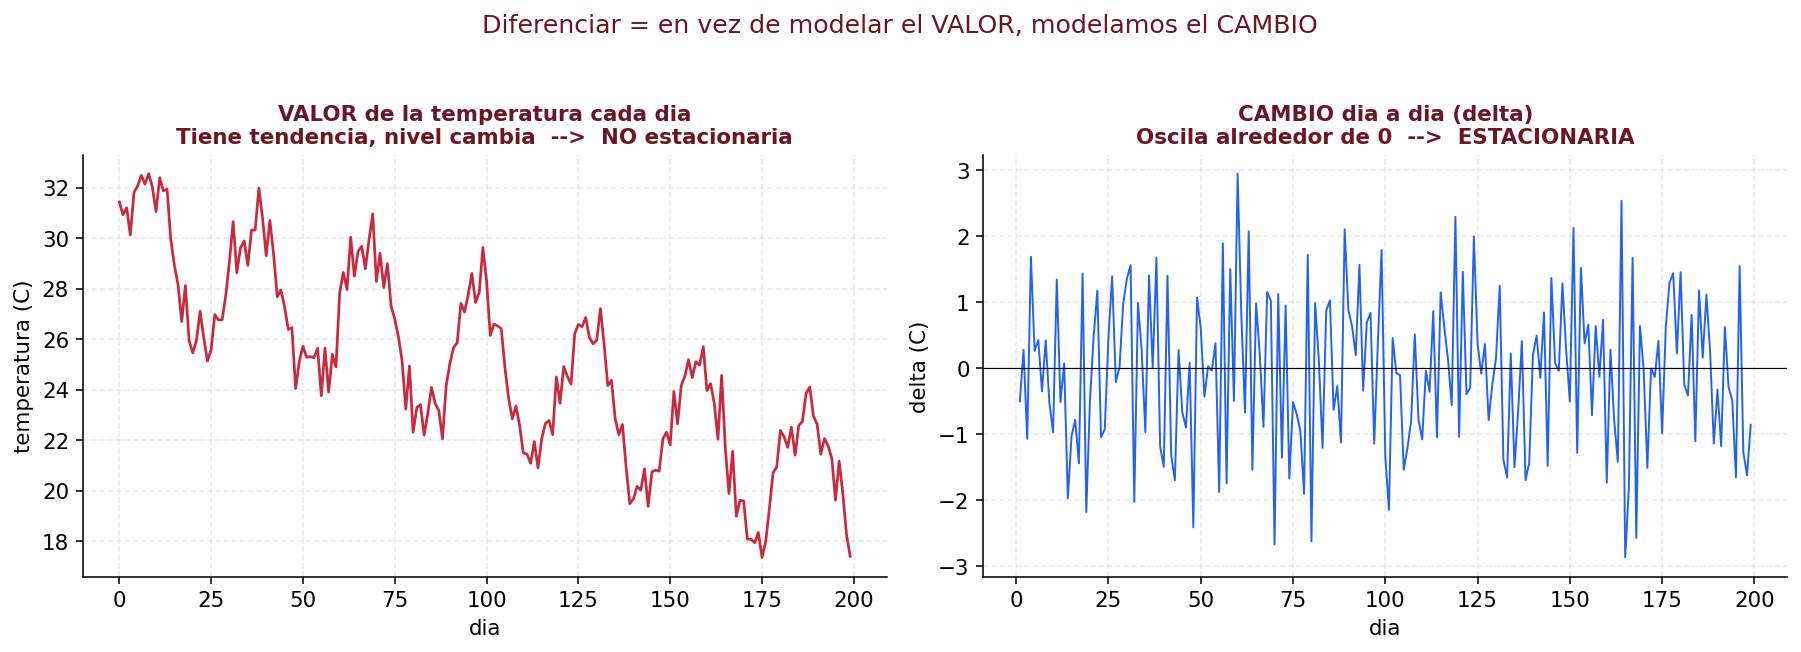
\includegraphics[width=0.97\textwidth]{fig_dif_intuicion.png}
  \end{center}
  \vspace{4pt}
  \begin{tcolorbox}[colback=arcaGray, colframe=arcaRed, leftrule=3pt,
    boxrule=0pt, sharp corners, left=8pt, right=8pt, top=4pt, bottom=4pt]
    {\footnotesize\color{arcaDark}
    El valor de la temperatura tiene tendencia (cae lento) y oscilaciones (estaciones).
    Pero el \emph{cambio} dia a dia oscila alrededor de cero con varianza estable.
    \textbf{Diferenciar = predecir el delta, no el nivel.}}
  \end{tcolorbox}
\end{frame}

\begin{frame}[shrink]{Tres tipos de diferenciacion --- cada una ataca una patologia}
  \vspace{4pt}
  \begin{itemize}\setlength{\itemsep}{8pt}
    \small
    \item[\textbf{1.}] \textbf{Tomar logaritmo:}\quad $\log(y_t)$\par
    {\footnotesize\color{textMuted}Estabiliza la VARIANZA cuando crece con el nivel
    (ventas, precios, poblacion).}
    \item[\textbf{2.}] \textbf{Diferencia regular:}\quad $\Delta y_t = y_t - y_{t-1}$\par
    {\footnotesize\color{textMuted}Quita la TENDENCIA (lineal o suave).}
    \item[\textbf{3.}] \textbf{Diferencia estacional:}\quad $\Delta_s y_t = y_t - y_{t-s}$\par
    {\footnotesize\color{textMuted}Quita la ESTACIONALIDAD de paso $s$
    (ej. $s=12$ para mensual con patron anual).}
  \end{itemize}
  \vspace{8pt}
  \begin{tcolorbox}[colback=arcaRed!8, colframe=arcaRed, leftrule=3pt,
    boxrule=0pt, sharp corners, left=8pt, right=8pt, top=4pt, bottom=4pt]
    {\footnotesize\color{arcaDark}\bfseries
    Se pueden combinar: $\Delta_{12} \Delta \log(y)$ aplica las tres en orden.
    Esto es lo que hace Prophet internamente cuando detecta no-estacionariedad.}
  \end{tcolorbox}
\end{frame}

\begin{frame}[shrink]{Aplicacion paso a paso sobre AirPassengers}
  \begin{center}
    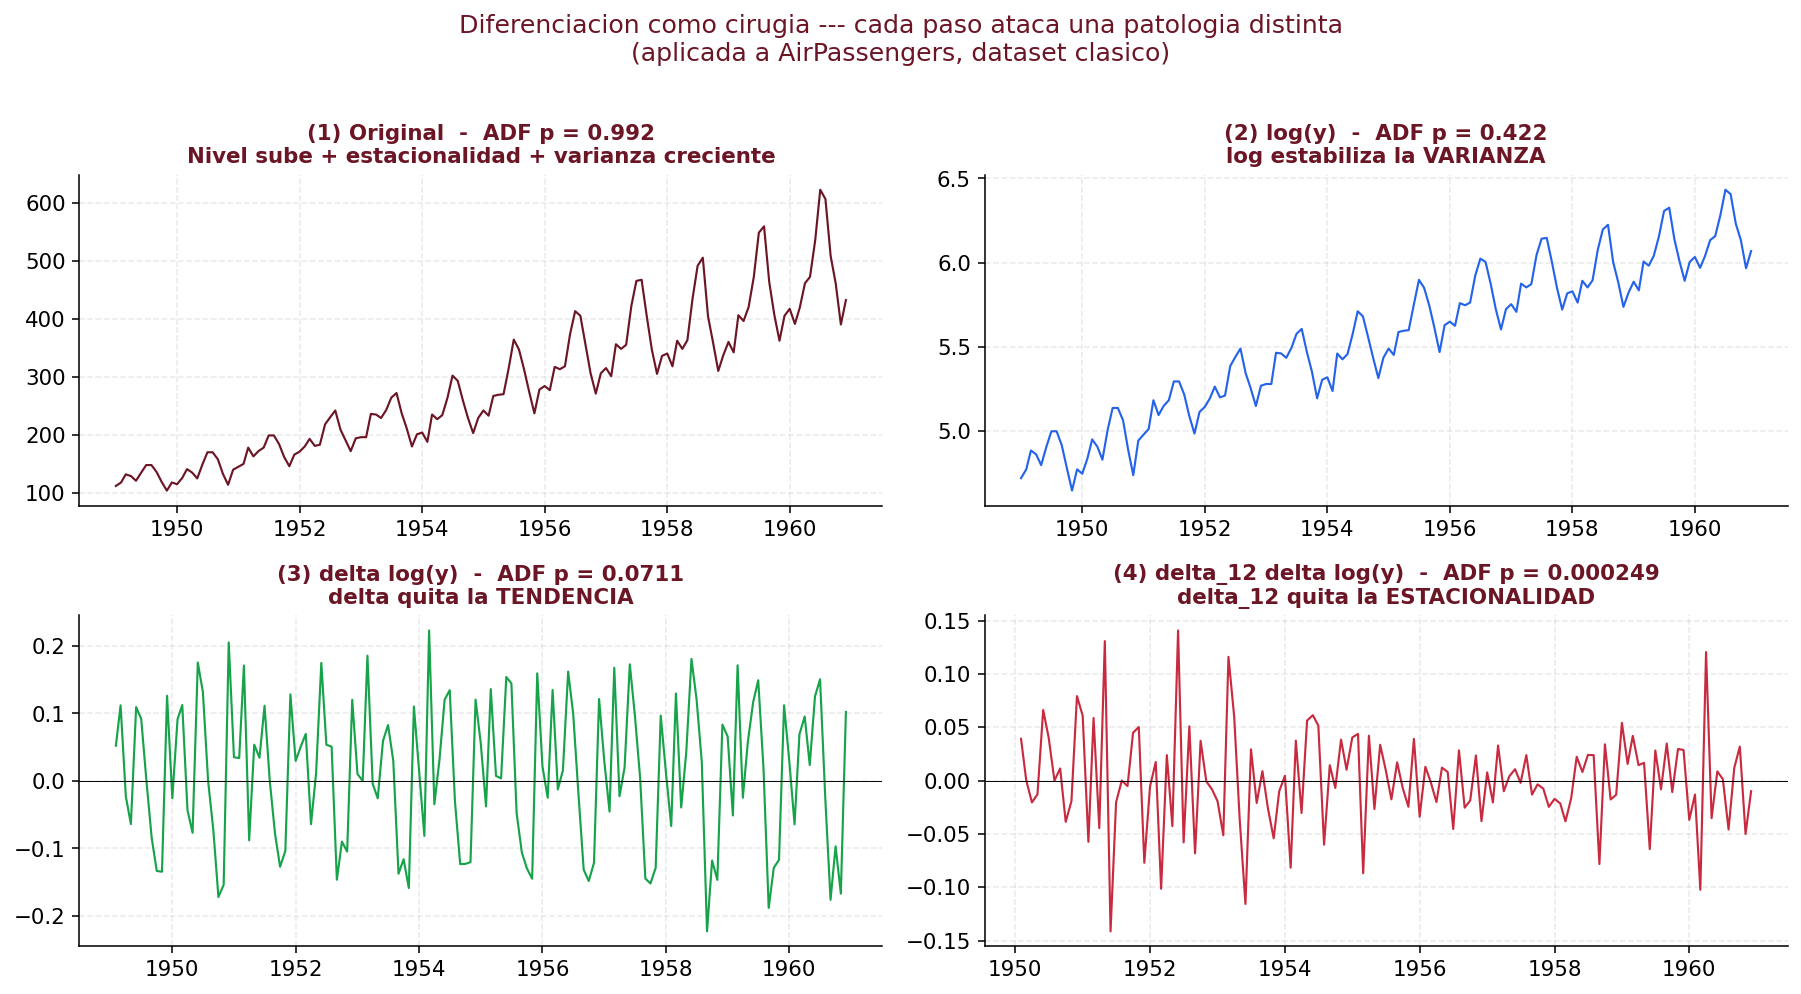
\includegraphics[width=0.97\textwidth]{fig_dif_airpass.png}
  \end{center}
  \vspace{2pt}
  {\footnotesize\color{arcaDark}
  ADF p baja en cada paso: $0.992 \to 0.422 \to 0.071 \to 0.0002$.
  Despues de las dos diferenciaciones, la serie es \textbf{claramente estacionaria}
  y podemos modelarla.}
\end{frame}

% =============================================================================
%  BLOQUE 3 - PROPHET SOBRE AIRPASSENGERS
% =============================================================================
\sectionframe{Bloque 3}{Prophet en accion\\(AirPassengers, el dataset clasico)}

\begin{frame}[shrink]{Por que Prophet --- el problema que resuelve}
  \begin{tcolorbox}[colback=arcaGray, colframe=arcaRed, leftrule=3pt,
    boxrule=0pt, sharp corners, left=8pt, right=8pt, top=6pt, bottom=6pt]
    {\small\color{arcaDark}
    Prophet (Facebook, 2017) fue disenado para series de \textbf{datos de negocio}:\par}
    \begin{itemize}\setlength{\itemsep}{2pt}
      \footnotesize
      \item Multiples estacionalidades (diaria, semanal, anual).
      \item Eventos especiales (navidad, dia del trabajador, black friday).
      \item Missing values y observaciones irregulares.
      \item Cambios de tendencia (changepoints automaticos).
    \end{itemize}
  \end{tcolorbox}
  \vspace{6pt}
  {\footnotesize\color{arcaDark}
  Descompone la serie en:\par}
  \[
    y(t) = g(t) + s(t) + h(t) + \varepsilon_t
  \]
  \vspace{-6pt}
  {\footnotesize\color{arcaDark}
  donde $g$ es tendencia con changepoints, $s$ es estacionalidad via Fourier,
  $h$ son holidays, y $\varepsilon$ es el ruido.}
\end{frame}

\begin{frame}[shrink]{Nuestra serie de prueba --- AirPassengers}
  \begin{center}
    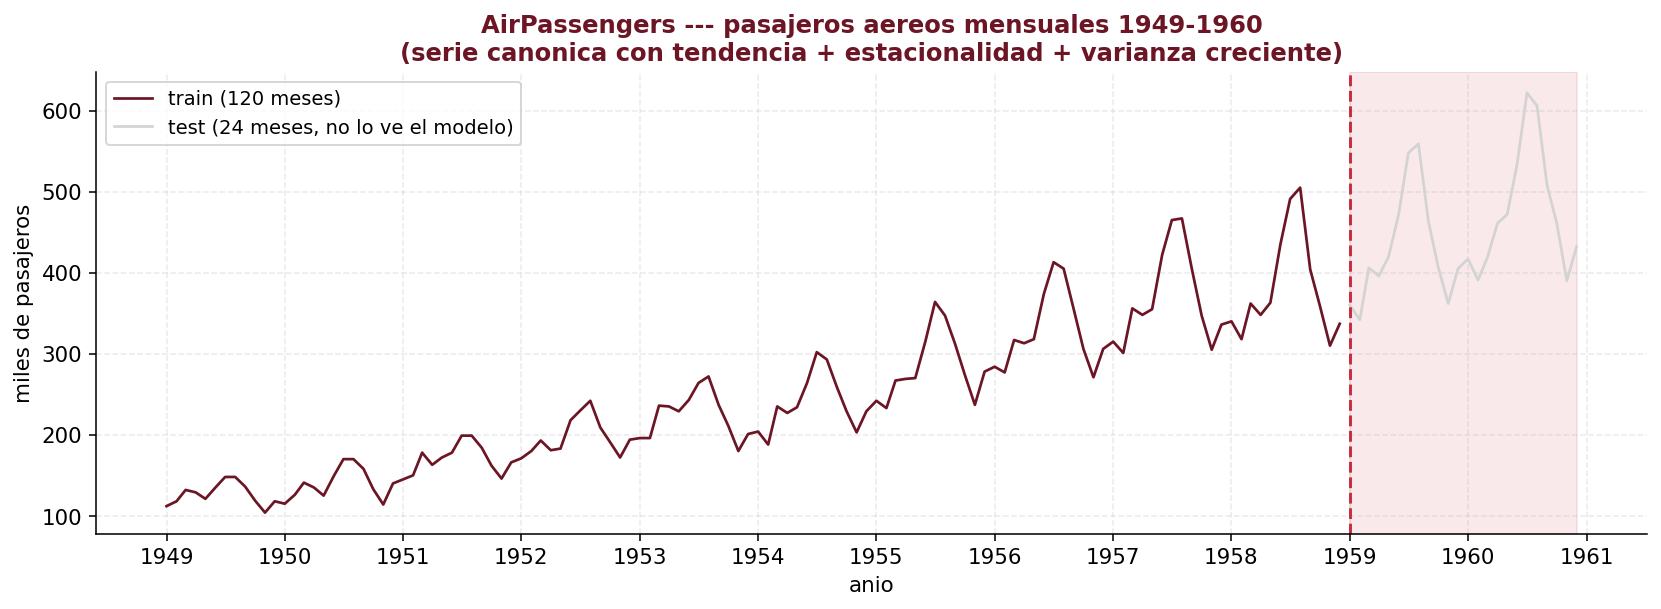
\includegraphics[width=0.97\textwidth]{fig_airpass_intro.png}
  \end{center}
  \vspace{2pt}
  {\footnotesize\color{arcaDark}
  Dataset canonico: pasajeros aereos mensuales 1949-1960. Tiene los tres
  ingredientes clasicos: \textbf{tendencia creciente}, \textbf{estacionalidad anual fuerte},
  \textbf{varianza creciente}. Train: 10 anios. Test: ultimos 24 meses.}
\end{frame}

\begin{frame}[fragile, shrink]{Prophet en codigo --- la API minima}
  \begin{pyblock}
from prophet import Prophet

df = pd.DataFrame({"ds": serie.index, "y": serie.values})

m = Prophet(yearly_seasonality=True,
            interval_width=0.80)
m.fit(df)

future = m.make_future_dataframe(periods=24, freq="MS")
forecast = m.predict(future)
# forecast tiene: yhat (punto), yhat_lower, yhat_upper (banda 80%)
  \end{pyblock}
  \vspace{4pt}
  {\footnotesize\color{arcaDark}
  Prophet espera columnas \texttt{ds} (fecha) e \texttt{y} (valor). La API es deliberadamente
  minima --- en 4 lineas tienes un forecast con bandas calibradas.}
\end{frame}

\begin{frame}[shrink]{El resultado --- Prophet acerta los picos estacionales}
  \begin{center}
    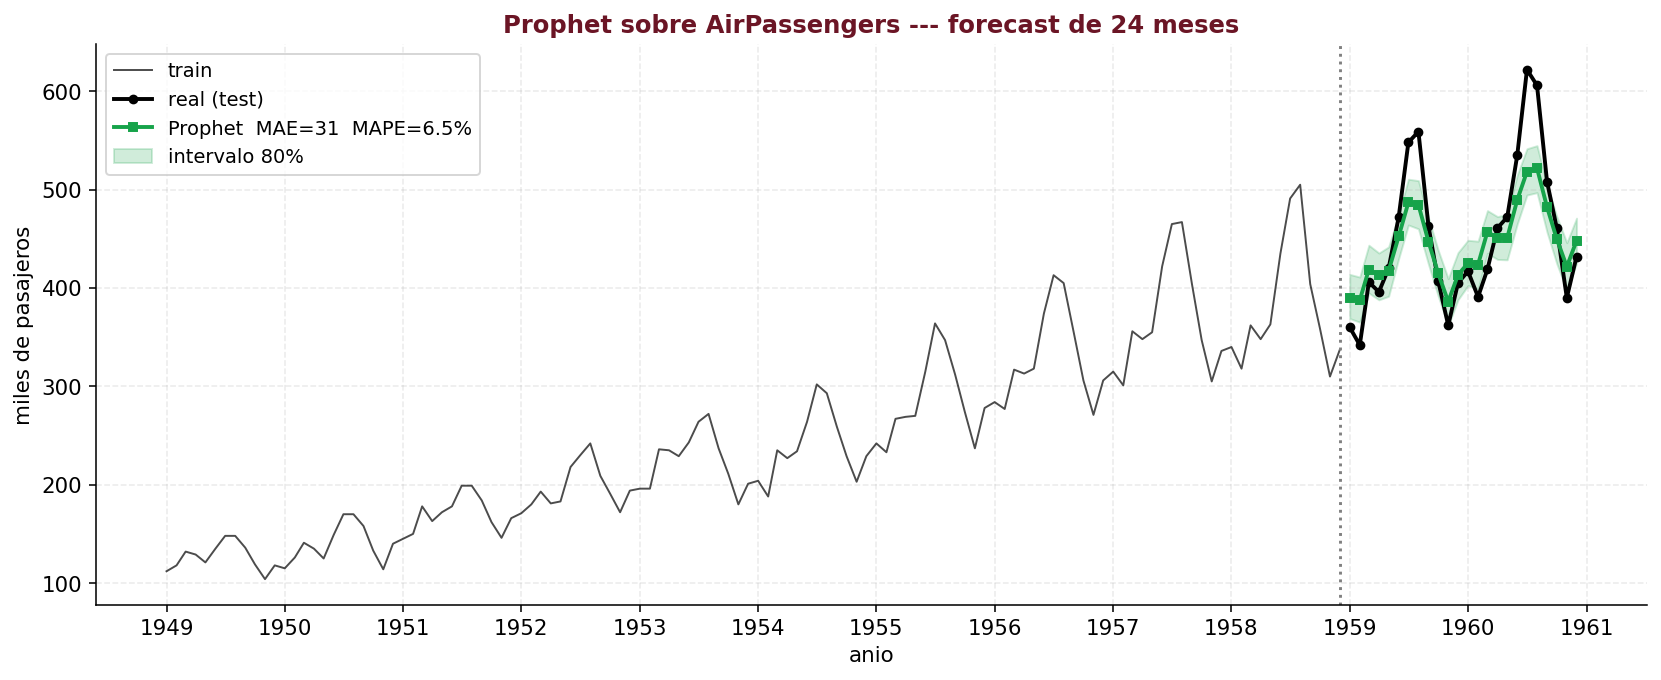
\includegraphics[width=0.97\textwidth]{fig_prophet_forecast_airpass.png}
  \end{center}
  \vspace{2pt}
  {\footnotesize\color{arcaDark}
  MAPE $6.5\%$ a horizonte de 2 anios. Prophet captura la tendencia y la oscilacion
  anual. Las bandas son su \textbf{intervalo de confianza nativo} (MCMC sobre los parametros).}
\end{frame}

\begin{frame}[shrink]{Lo que Prophet aprendio por dentro --- componentes interpretables}
  \begin{center}
    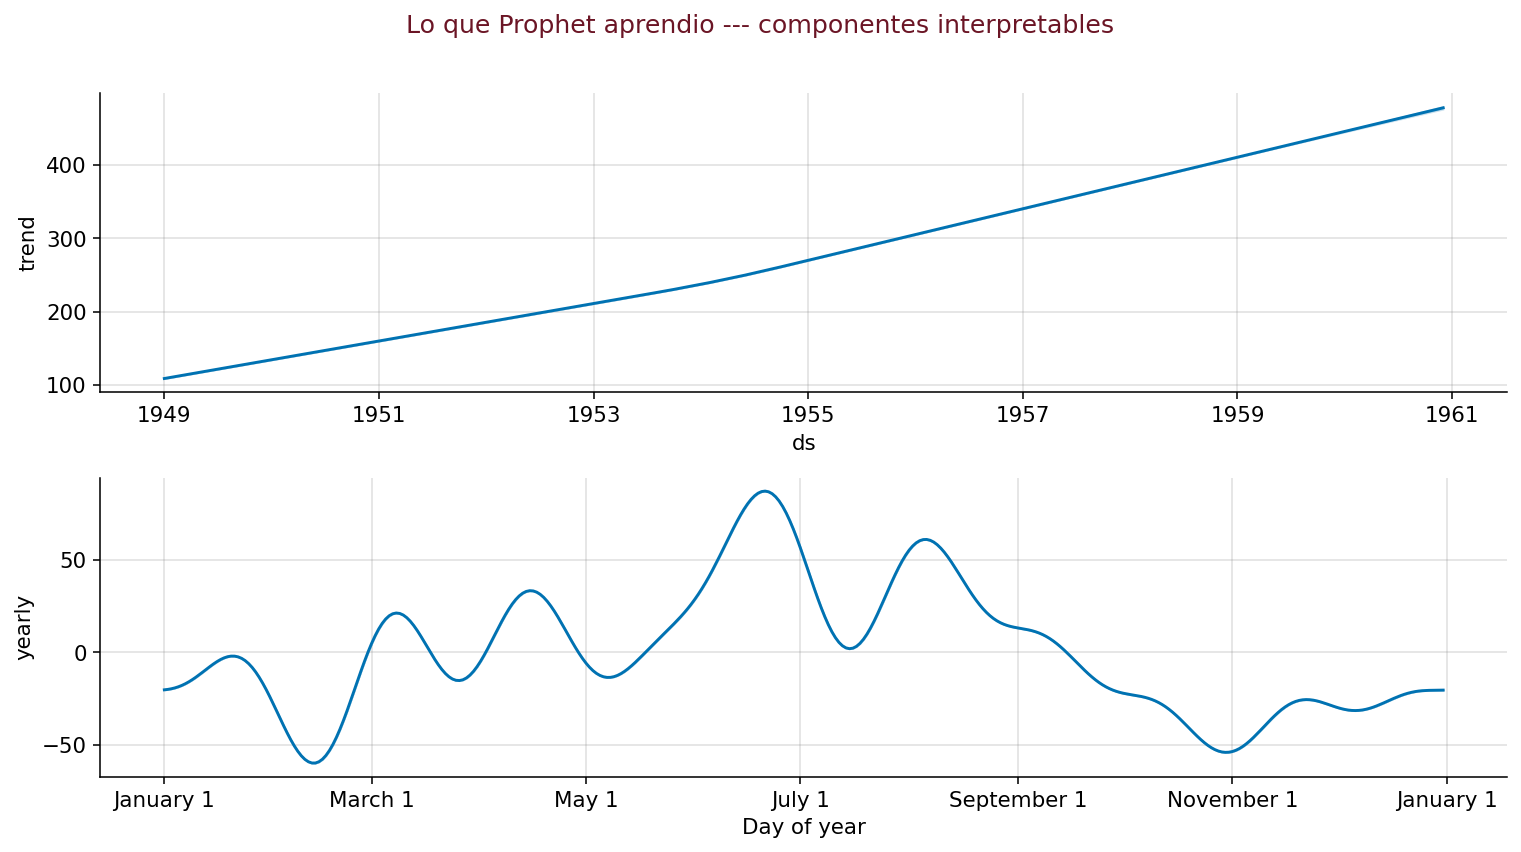
\includegraphics[width=0.88\textwidth]{fig_prophet_components_airpass.png}
  \end{center}
  \vspace{2pt}
  {\footnotesize\color{arcaDark}
  A diferencia de modelos blackbox, Prophet te muestra las piezas: tendencia,
  estacionalidad anual. Util cuando hay que \emph{explicarle al jefe} por que el modelo
  dice lo que dice.}
\end{frame}

% =============================================================================
%  BLOQUE 4 - METRICAS
% =============================================================================
\sectionframe{Bloque 4}{Metricas honestas\\(walk-forward + cuando usar cada metrica)}

\begin{frame}[shrink]{Walk-forward CV --- no podes shufflear el tiempo}
  \begin{tcolorbox}[colback=arcaRed!8, colframe=arcaRed, leftrule=3pt,
    boxrule=0pt, sharp corners, left=8pt, right=8pt, top=4pt, bottom=4pt]
    {\footnotesize\color{arcaDark}\bfseries
    En series temporales el orden importa. No podes usar el futuro para validar
    el pasado --- en produccion nunca lo vas a tener.}
  \end{tcolorbox}
  \vspace{6pt}
  \begin{center}
    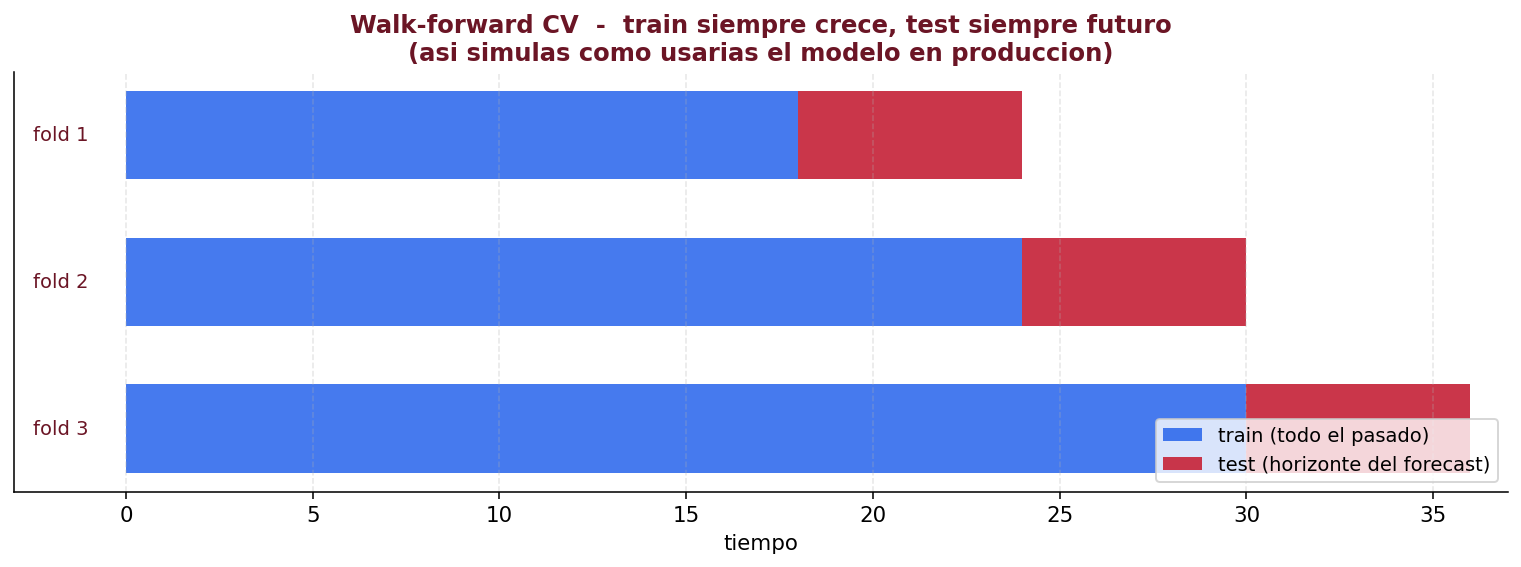
\includegraphics[width=0.85\textwidth]{fig_walkforward.png}
  \end{center}
  \vspace{2pt}
  {\footnotesize\color{arcaDark}
  Cada fold: entrenar con todo el pasado disponible hasta ese momento, predecir el
  horizonte, medir. Asi simulas como vas a usar el modelo en produccion.}
\end{frame}

\begin{frame}[shrink]{Cuatro metricas, cuatro usos distintos}
  \begin{center}
    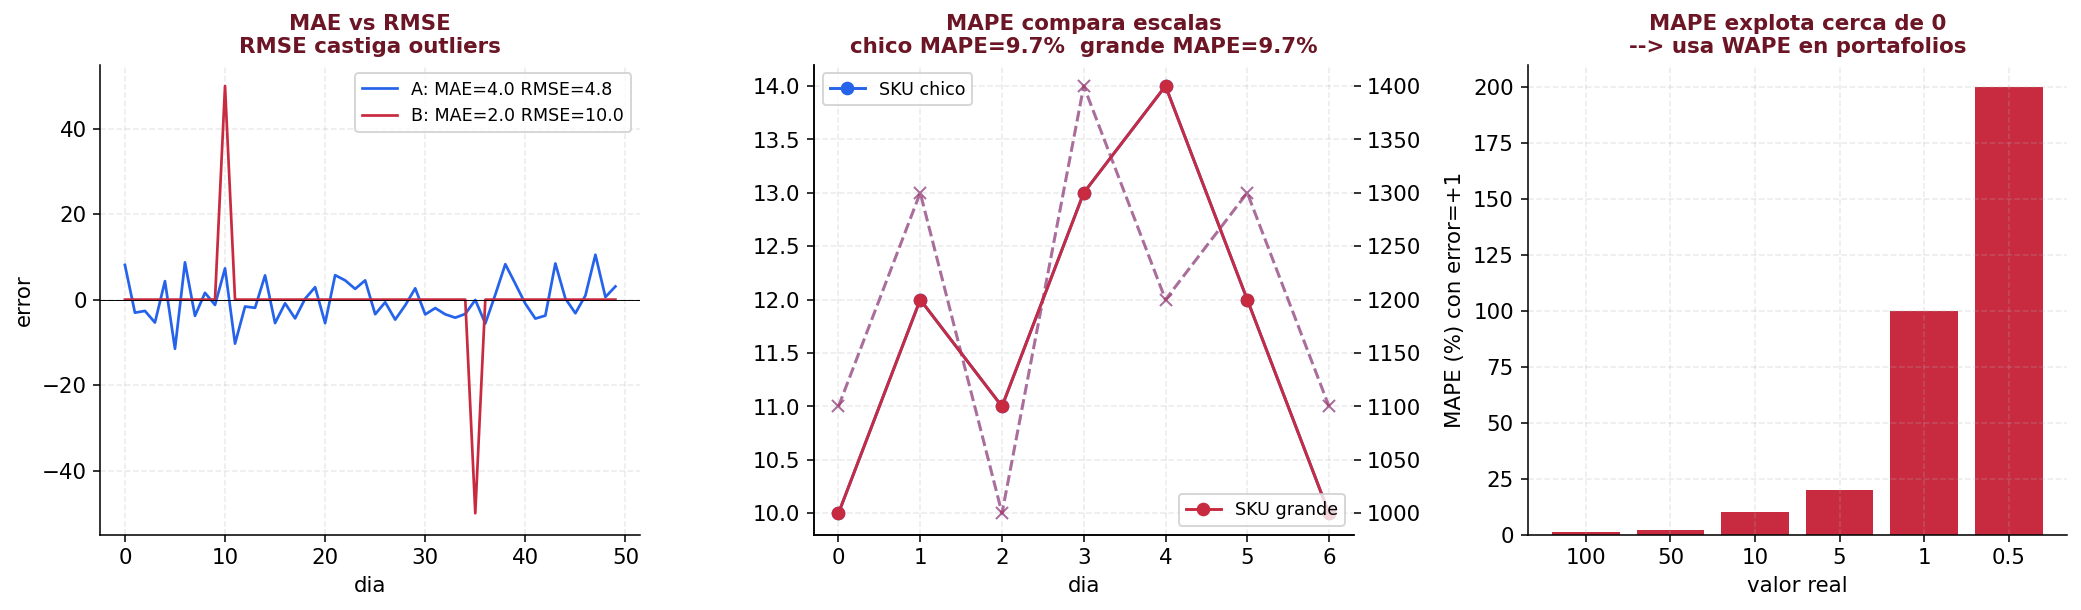
\includegraphics[width=0.97\textwidth]{fig_metricas_cuando.png}
  \end{center}
  \vspace{2pt}
  \begin{itemize}\setlength{\itemsep}{1pt}
    \footnotesize
    \item \textbf{MAE} (error absoluto medio): facil de interpretar, robusta a outliers.
    \item \textbf{RMSE} (raiz del cuadratico): castiga errores grandes ($\Rightarrow$ outliers).
    \item \textbf{MAPE} (\% error absoluto): compara escalas, pero \emph{explota cerca de 0}.
    \item \textbf{WAPE} (weighted abs percent): suma errores / suma reales. Metrica de portafolio.
  \end{itemize}
\end{frame}

\begin{frame}[shrink]{Cuatro modelos sobre los mismos 24 meses}
  \begin{center}
    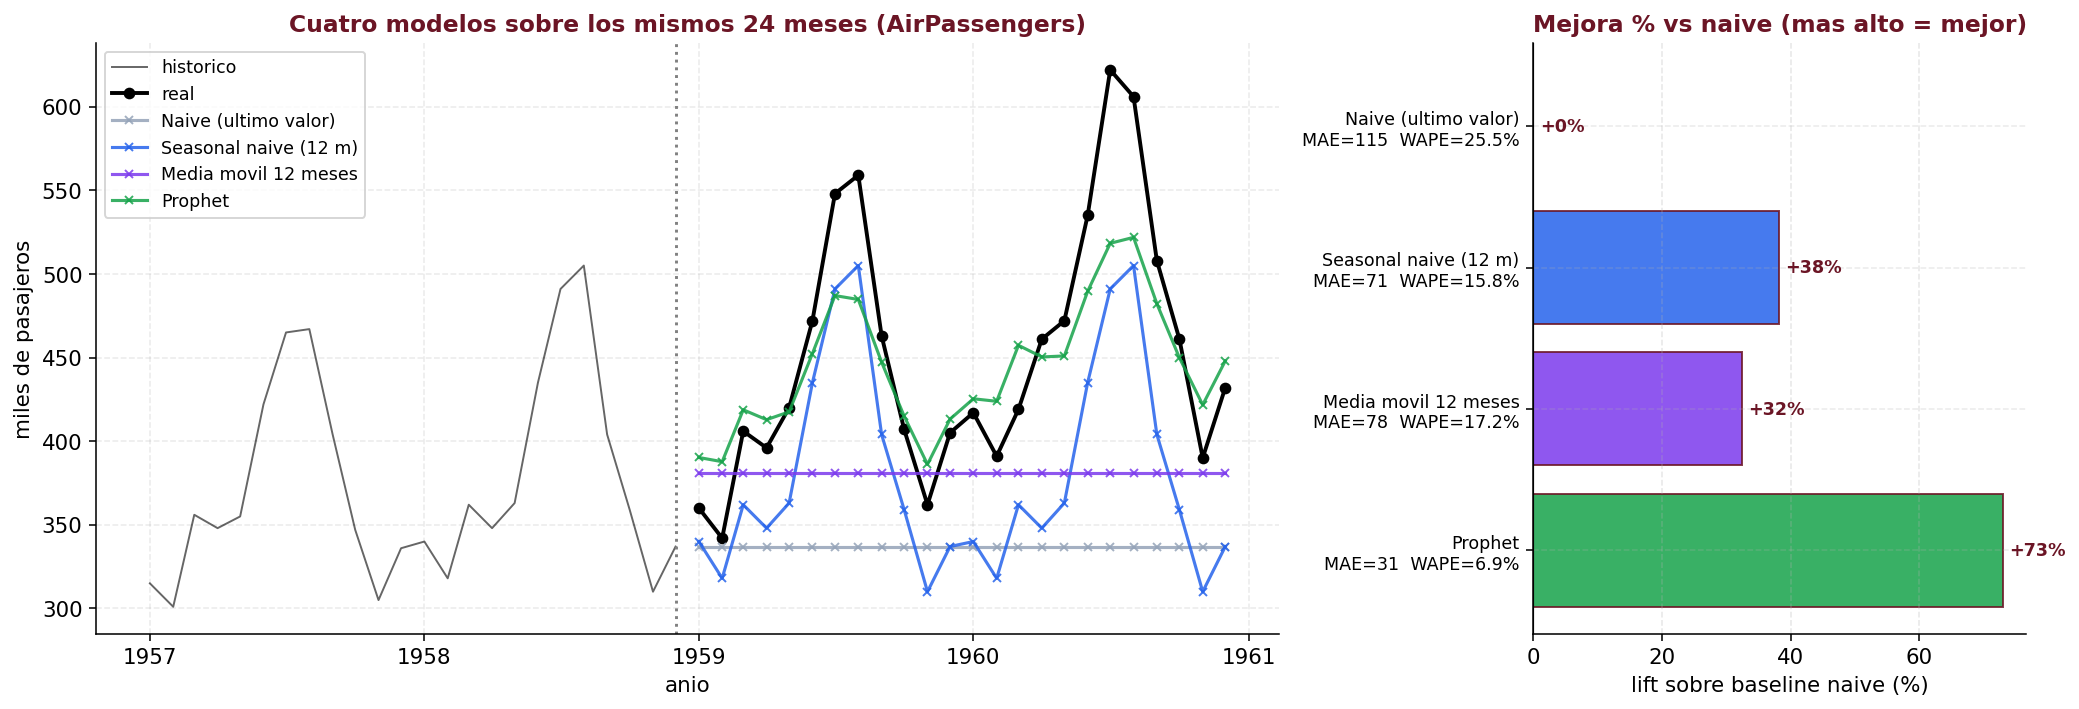
\includegraphics[width=0.97\textwidth]{fig_comparacion_airpass.png}
  \end{center}
  \vspace{2pt}
  \begin{tcolorbox}[colback=arcaRed!8, colframe=arcaRed, leftrule=3pt,
    boxrule=0pt, sharp corners, left=8pt, right=8pt, top=4pt, bottom=4pt]
    {\footnotesize\color{arcaDark}\bfseries
    Prophet gana con $+73\%$ de mejora sobre naive. Seasonal naive y MA tambien
    aportan, pero Prophet es claramente mejor cuando hay tendencia + estacionalidad.}
  \end{tcolorbox}
\end{frame}

% =============================================================================
%  BLOQUE 5 - INFERENCIA Y COSTO ASIMETRICO
% =============================================================================
\sectionframe{Bloque 5}{Inferencia --- la prediccion\\NO es el numero final}

\begin{frame}[shrink]{La prediccion es un RANGO, no un punto}
  \begin{center}
    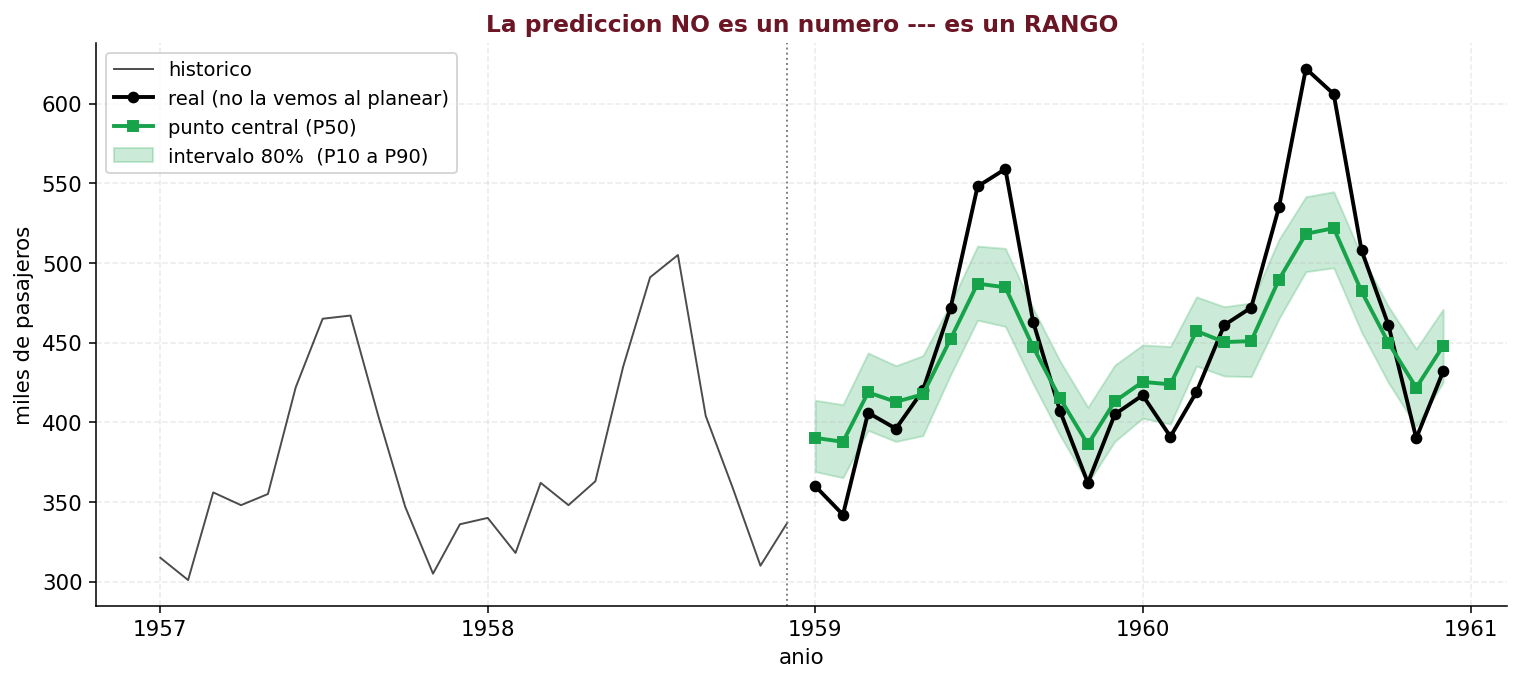
\includegraphics[width=0.95\textwidth]{fig_inferencia_intervalos.png}
  \end{center}
  \vspace{2pt}
  {\footnotesize\color{arcaDark}
  El punto verde es el centro (P50). La banda verde es el intervalo de $80\%$:
  el modelo dice ``hay $80\%$ de probabilidad de que la realidad caiga aqui''.}
\end{frame}

\begin{frame}[shrink]{Costo asimetrico --- el concepto que define la decision}
  \begin{center}
    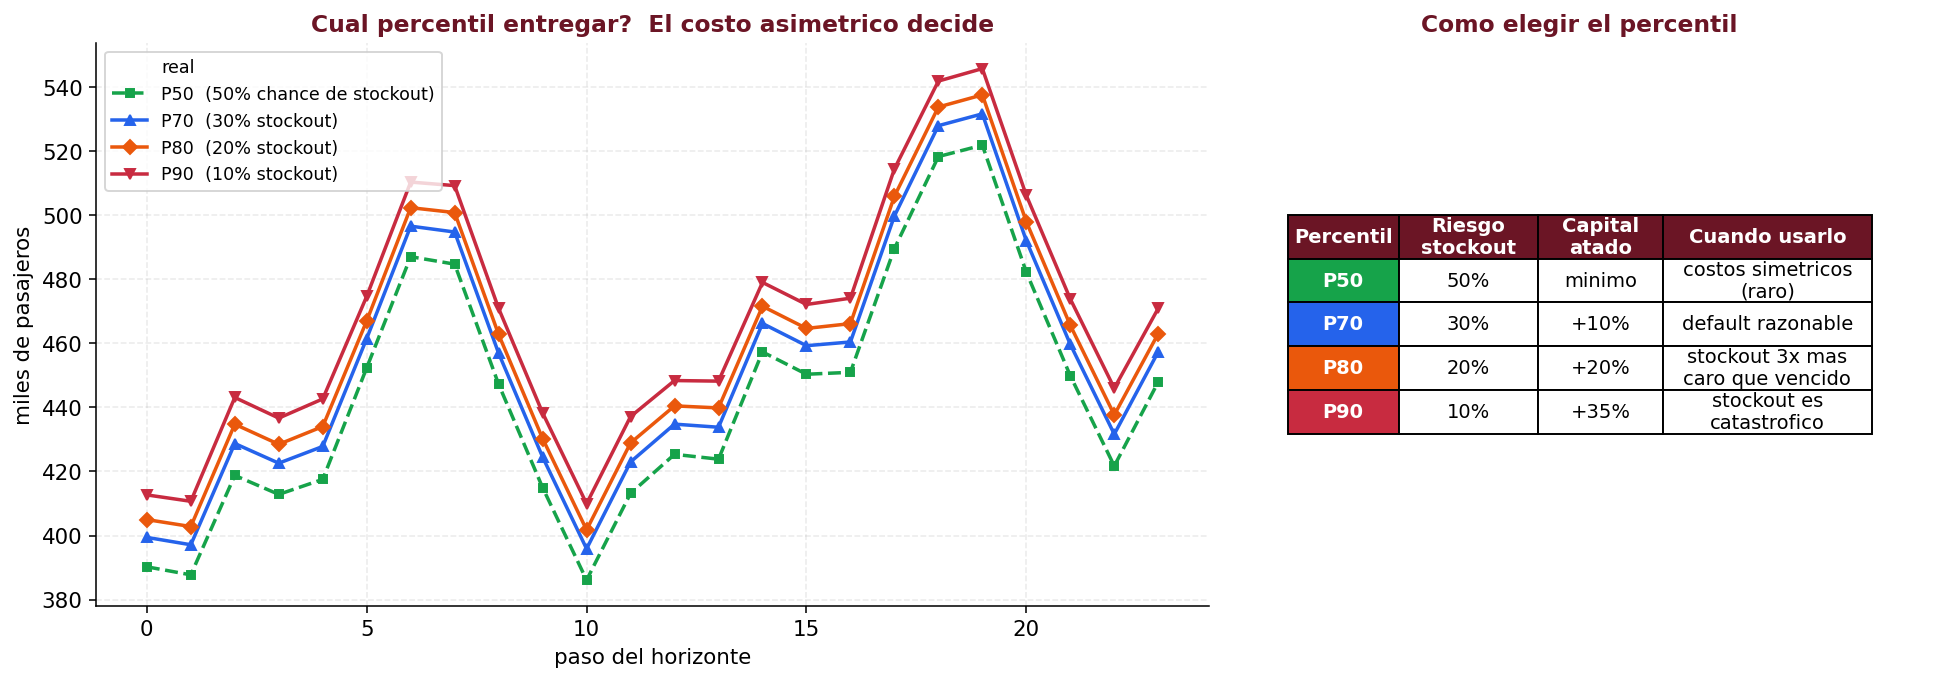
\includegraphics[width=0.97\textwidth]{fig_costo_asimetrico.png}
  \end{center}
  \vspace{2pt}
  \begin{tcolorbox}[colback=arcaRed!8, colframe=arcaRed, leftrule=3pt,
    boxrule=0pt, sharp corners, left=8pt, right=8pt, top=4pt, bottom=4pt]
    {\footnotesize\color{arcaDark}
    Si entregas el P50, vas a tener stockout el $50\%$ del tiempo.
    \textbf{El costo de stockout y de sobrestock NO es simetrico} $\Rightarrow$
    entregamos un percentil mas alto. La tabla muestra el tradeoff.}
  \end{tcolorbox}
\end{frame}

% =============================================================================
%  BLOQUE 6 - CASO APLICADO: FAVORITA
% =============================================================================
\sectionframe{Bloque 6}{Caso aplicado --- Favorita Quito Q44\\(6 meses de forecast con Prophet)}

\begin{frame}[shrink]{El caso real --- bebidas en una tienda Favorita}
  \begin{center}
    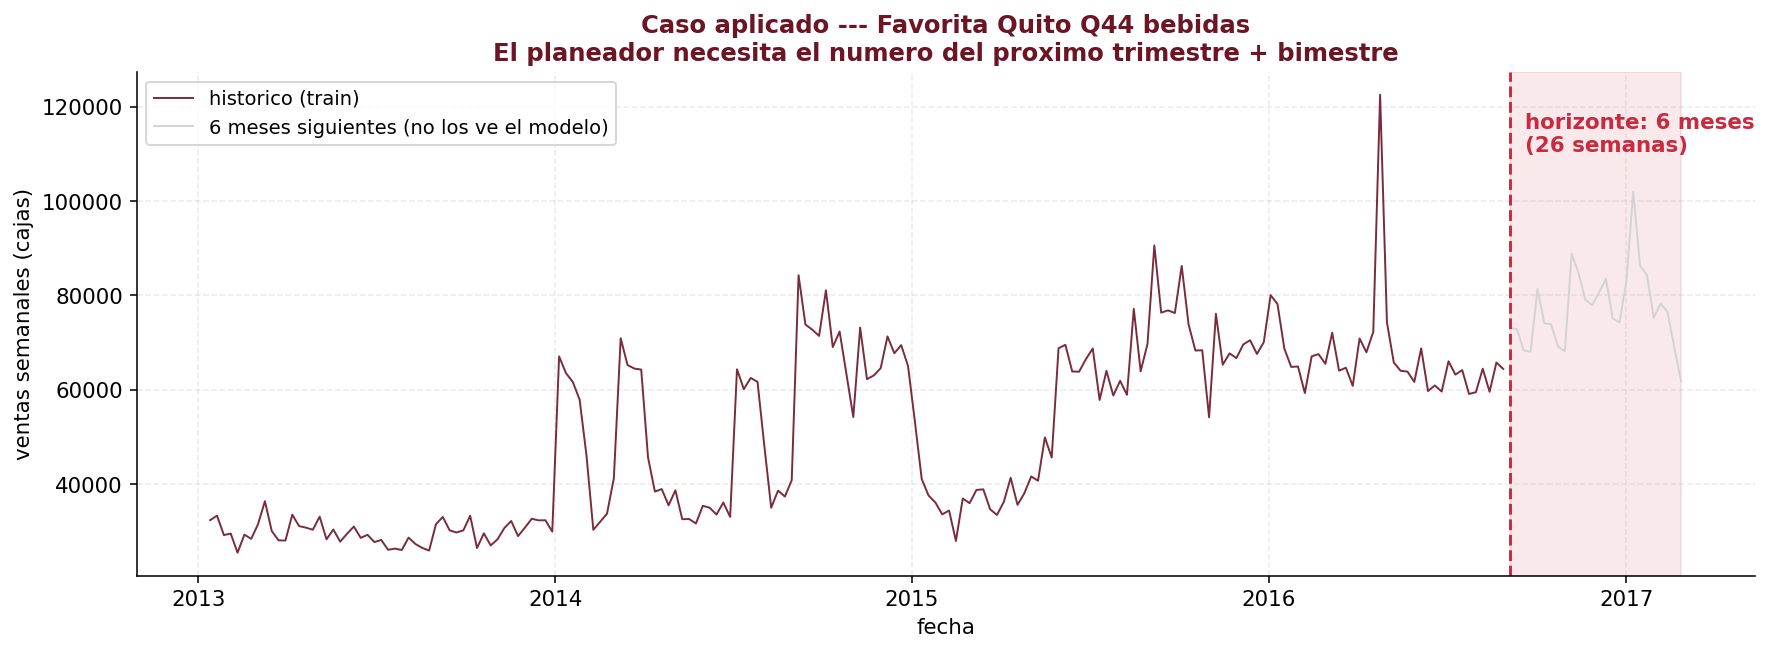
\includegraphics[width=0.97\textwidth]{fig_favorita_problema.png}
  \end{center}
  \vspace{2pt}
  {\footnotesize\color{arcaDark}
  Dataset real de Favorita Ecuador. Ventas semanales de la categoria
  \textbf{beverages} en una tienda de Quito (Q44). El planeador de Arca Continental
  necesita el numero para los proximos \textbf{6 meses} (26 semanas).}
\end{frame}

\begin{frame}[fragile, shrink]{Prophet con holidays Ecuador --- en codigo}
  \begin{pyblock}
from prophet import Prophet
import holidays

ec = holidays.country_holidays("EC", years=range(2013, 2018))
hdays = pd.DataFrame({
    "holiday": list(ec.values()),
    "ds":      pd.to_datetime(list(ec.keys())),
    "lower_window": 0, "upper_window": 1,
})

m = Prophet(yearly_seasonality=True, weekly_seasonality=False,
            holidays=hdays, interval_width=0.80)
m.fit(df_train)
forecast = m.predict(m.make_future_dataframe(periods=26, freq="W"))
  \end{pyblock}
  \vspace{2pt}
  {\footnotesize\color{arcaDark}
  Anadimos los holidays oficiales de Ecuador como regresor. Prophet va a aprender
  el efecto especifico de cada uno en las ventas.}
\end{frame}

\begin{frame}[shrink]{Forecast 6 meses --- Prophet sobre la serie real}
  \begin{center}
    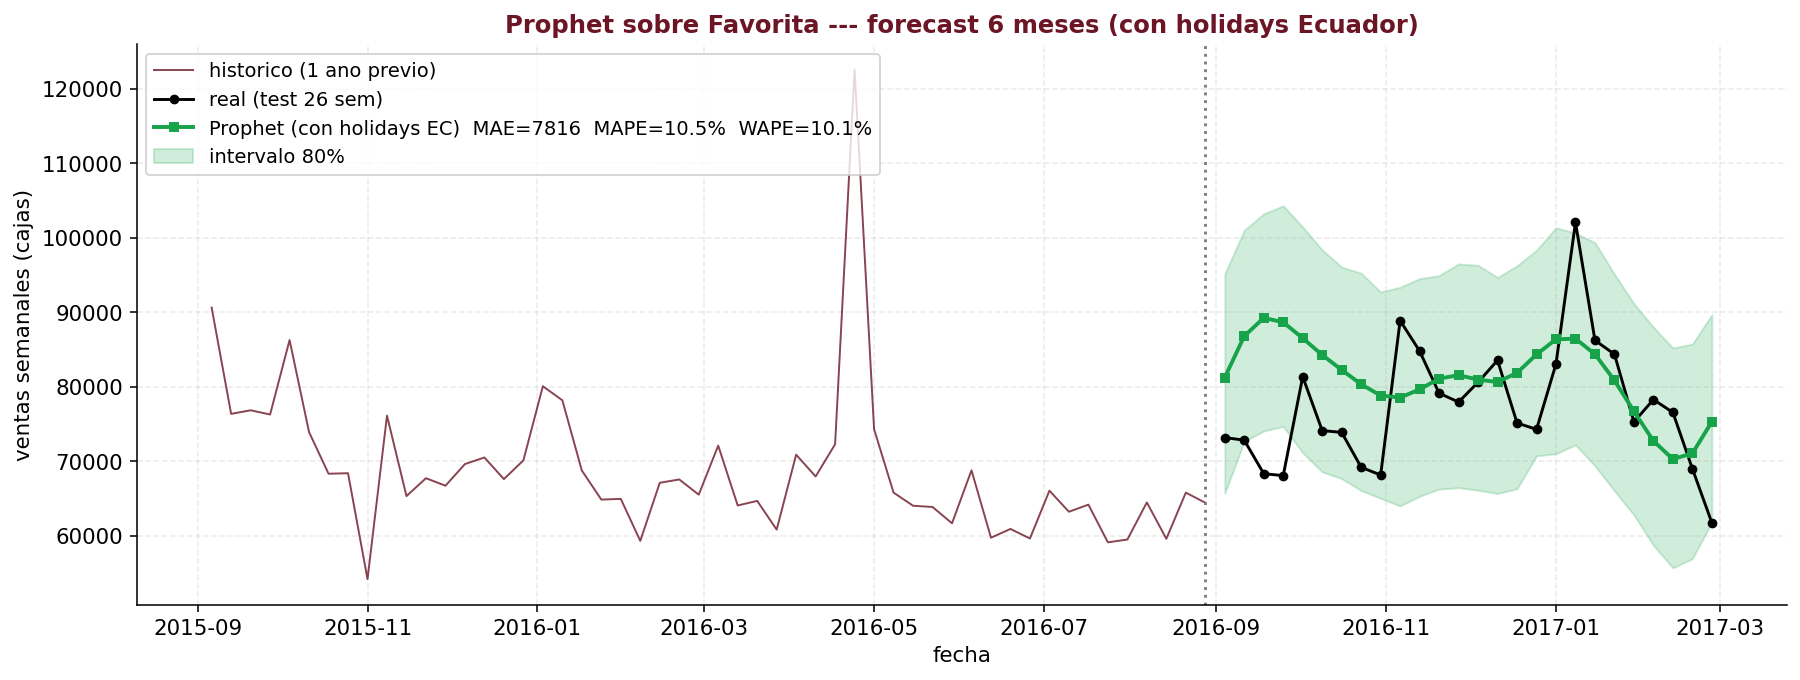
\includegraphics[width=0.97\textwidth]{fig_favorita_prophet.png}
  \end{center}
  \vspace{2pt}
  \begin{tcolorbox}[colback=arcaRed!8, colframe=arcaRed, leftrule=3pt,
    boxrule=0pt, sharp corners, left=8pt, right=8pt, top=4pt, bottom=4pt]
    {\footnotesize\color{arcaDark}\bfseries
    WAPE $\sim 10\%$ a horizonte de 6 meses sobre una serie real con ruido,
    tendencia creciente y eventos. En forecasting de demanda industrial,
    eso es un excelente resultado.}
  \end{tcolorbox}
\end{frame}

\begin{frame}[shrink]{Que aprendio Prophet sobre las ventas de Favorita}
  \begin{center}
    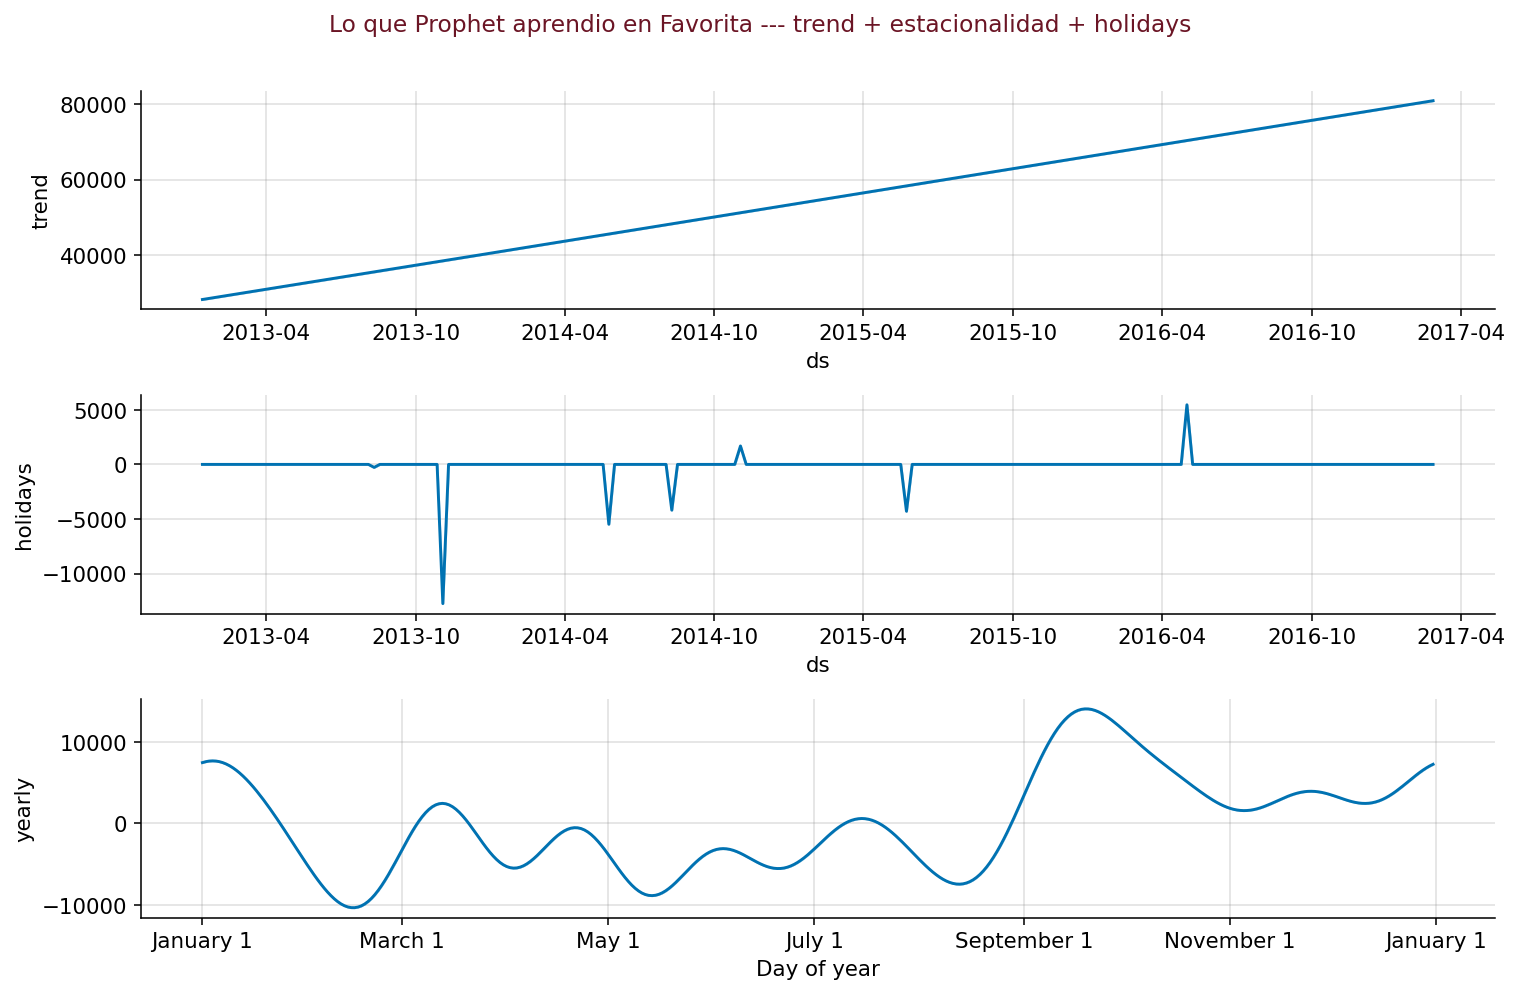
\includegraphics[width=0.88\textwidth]{fig_favorita_components.png}
  \end{center}
  \vspace{2pt}
  {\footnotesize\color{arcaDark}
  \textbf{Tendencia:} crecimiento sostenido de $\sim 30$k a $\sim 80$k semanal (3x en 4 anios).
  \textbf{Holidays:} algunos feriados bajan las ventas $\sim 5$-$12$k.
  \textbf{Patron anual:} pico en septiembre, minimo en febrero.}
\end{frame}

% =============================================================================
%  BLOQUE 7 - CIERRE
% =============================================================================
\sectionframe{Bloque 7}{Cierre --- decision tree\\y que viene en clase 33}

\begin{frame}[shrink]{Cuando usar cada modelo --- la guia practica}
  \begin{center}
    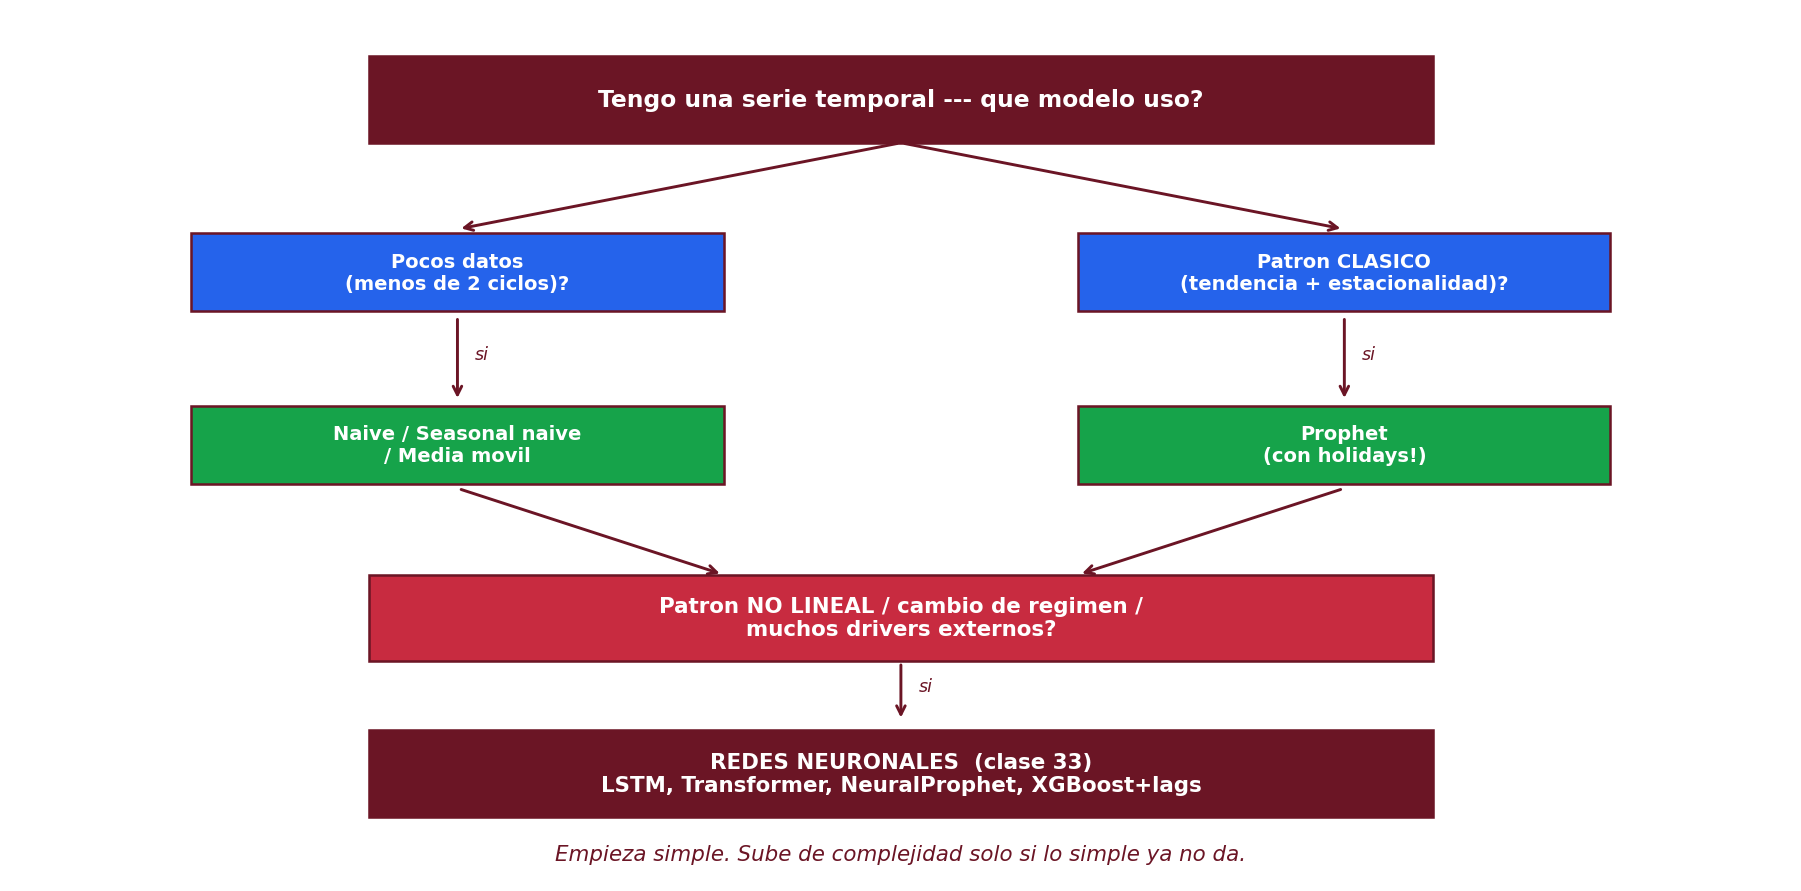
\includegraphics[width=0.92\textwidth]{fig_decision_tree.png}
  \end{center}
\end{frame}

\begin{frame}[shrink]{Lo que te llevas de la clase de hoy}
  \begin{itemize}\setlength{\itemsep}{6pt}
    \footnotesize
    \item Una serie tiene que ser \textbf{estacionaria} para que un modelo aprenda algo util.
    Si no lo es, diferenciamos.
    \item \textbf{ADF} diagnostica. Tres transformaciones (log, $\Delta$, $\Delta_s$)
    cubren la mayoria de casos.
    \item \textbf{Prophet} es la herramienta moderna para datos de negocio con tendencia,
    estacionalidad y holidays. API minima, componentes interpretables.
    \item \textbf{Walk-forward CV} para metricas honestas. \textbf{MAE, RMSE, MAPE, WAPE}
    cada una con su uso especifico.
    \item \textbf{La prediccion es un rango, no un punto.} El \textbf{costo asimetrico}
    decide el percentil que entregas.
    \item Cuando los clasicos no bastan (regimen cambia, no-linealidad, multivariado):
    \textbf{redes neuronales (clase 33)}.
  \end{itemize}

  \vspace{6pt}
  \begin{tcolorbox}[colback=arcaRed!8, colframe=arcaRed, leftrule=3pt,
    boxrule=0pt, sharp corners, left=8pt, right=8pt, top=4pt, bottom=4pt]
    {\small\color{arcaDark}\bfseries
    Proxima clase: redes neuronales para series temporales
    (LSTM, Transformer, NeuralProphet) --- para los casos donde los clasicos se quedan cortos.}
  \end{tcolorbox}
\end{frame}

\begin{frame}[plain, noframenumbering]
  \begin{tikzpicture}[remember picture, overlay]
    \fill[arcaDark] (current page.south west) rectangle (current page.north east);
    \node[anchor=center, text=white, font=\Huge\bfseries] at
      ([yshift=1cm]current page.center) {Gracias};
    \node[anchor=center, text=white!85, font=\Large] at
      ([yshift=-0.2cm]current page.center) {Preguntas?};
    \node[anchor=center, text=white!70, font=\small] at
      ([yshift=-1.5cm]current page.center)
      {Codigo + datos: github.com/cmosquerat/arca-diplomado/tree/main/clase-32};
  \end{tikzpicture}
\end{frame}

\end{document}
